\documentclass[usetikz]{style/cepcnote}
%\usepackage{cepcphysics} % Contains useful shortcuts. Uncomment to use
                           % See instruction.pdf for details
\skipbeforetitle{100pt}
\title{Optimization for CEPC vertex}

% Author
%if not given, typesets ``The CEPC collaboration''
%\author{The CEPC Collaboration}
% if multiple authors/affiliations are needed, use the authblk package
\usepackage{authblk}
\usepackage{subfigure}
\renewcommand\Authands{, } % avoid ``. and'' for last author
\renewcommand\Affilfont{\itshape\small} % affiliation formatting

\author[a,b]{Zhigang Wu}
\author[a]{Gang Li}
\affil[a]{Institude of High Energy Physics, CAS}
\affil[b]{University of Chinese Academy of Science}

% Date: if not given, uses current date
%\date{\today}

\draftversion{1.0}
 
\mail  {wuzg@mail.ihep.ac.cn}
\cepcnote{CEPC-DET-OPTI-2017-001}

\abstracttext{
The vertex detector plays a key role for the reconstruction of secondary vertices and flavor tagging of $b$-/$c$-quark jets and $\tau$-lepton. Under the framework of Mokka and Marlin, full simulation has been done to improve the performance of vertex. In detail, we scan the different values of material budget, spatial resolution and inner radius, and study the performance variation through ROC curve. In general, these optimizations improve c-tagging significantly, while have small influence on b-tagging.
}
%%%%%%%%%%%%%%%%%%%%%%%%%%%%%%%%%%%%
%            Content               % 
%%%%%%%%%%%%%%%%%%%%%%%%%%%%%%%%%%%%

\begin{document}

\section{Introduction}

High Energy Circular Electron Positron Collider (CEPC) works as a “Higgs” factory to measure Higgs boson precisely. For the channel of $H->b\overline{b}, c\overline{c}, g\overline{g}$, vertex detector plays a key role in flavor tagging and decides the accuracy of measurement. The optimization of detector position and structure needs to be done to get a better performance. We have aimed on the material budget, spatial resolution and inner radius of vertex through full simulation based on Mokka and Marlin. For detector model, cepc\_v1 default setting is used. For digitization, a simple Gaussian smearing is used. For reconstruction, xxx. ROC curve is a common way to show the power of flavor-tagging. In general, the bigger the area between ROC curve and coordinate axis is, the more powerful flavor tagging is. In this note, we show the ROC curves of different quarks versus different parameters and how much it effects the flavor tagging performance. 

\section{Results}

\subsection{Material budget}

In event selection, we choose $50000\ z->b\overline{b}, 50000\ z->c\overline{c}, 50000\ z->l\overline{l}\ (uds\ pairs)$ as the generator (location is /home/bes/lig/higgs/data/Fast\_Simulation/wo\_beamstruhlung/background/Z-pole/). After Geant4 simulation, digitization, reconstruction, jetclustering, and training, we get the final states of b, c, and uds pairs. Here we show a worst correlation matrixs and two pictures of train and test results in the simulation of baseline design. From the figure \ref{fig:cor_mar} and figure \ref{fig:train_test}, we can see there are no unreasonable parameters and over-training phenomenon. 
\begin{figure}[!ht]
	\centering
	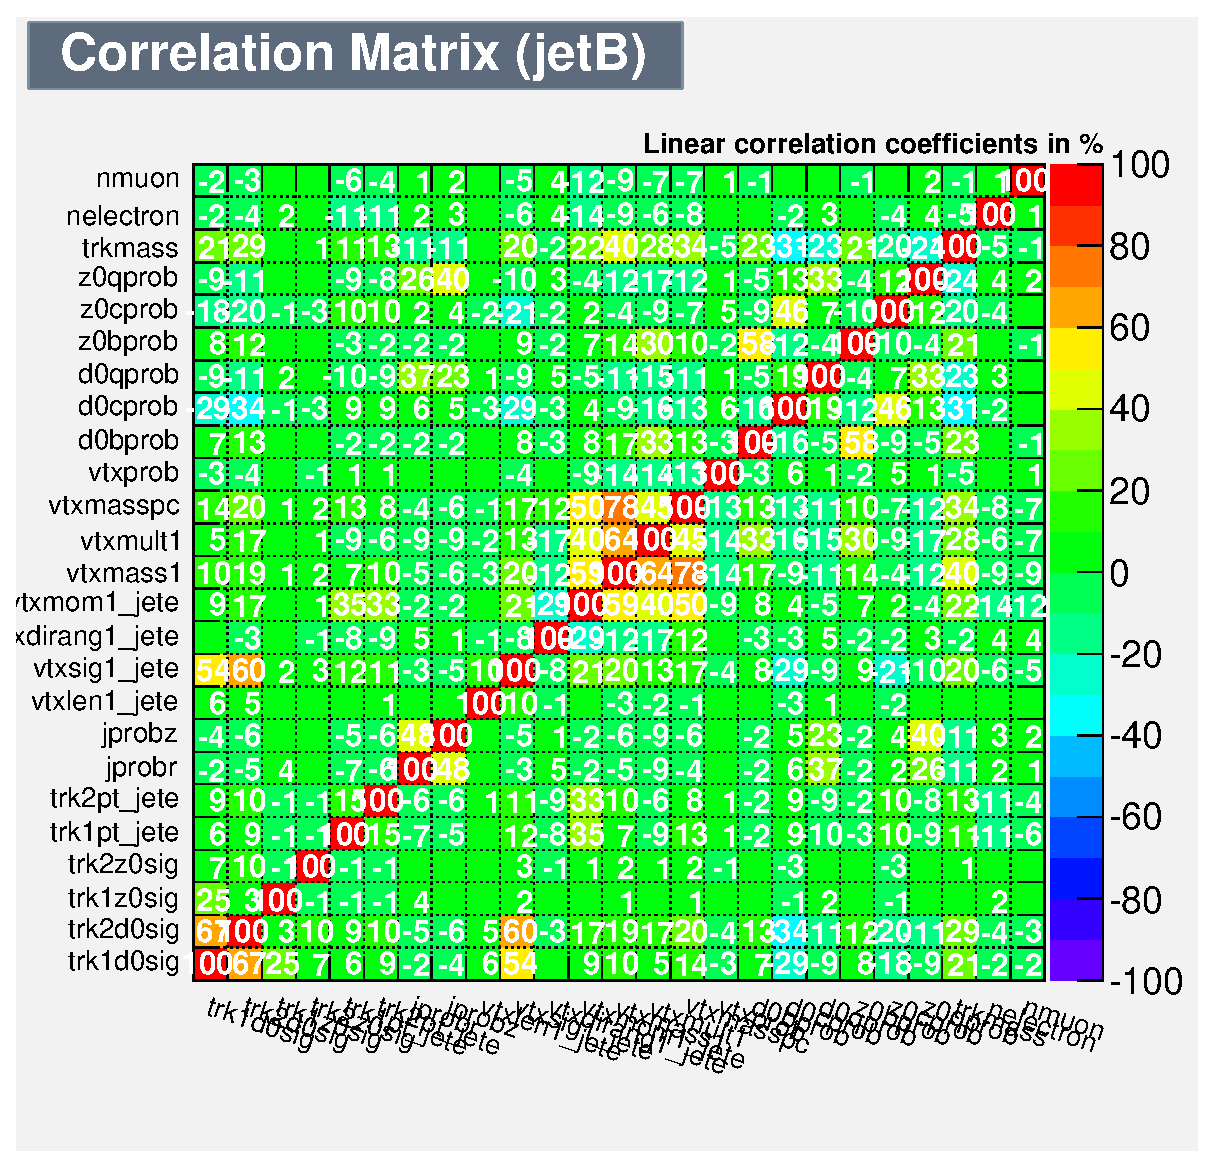
\includegraphics[scale=0.5]{figures/CorrelationMatrixjetB_c1.eps}
	\caption{worst correlation Matrix of jet B training}
	\label{fig:cor_mar}
\end{figure}

\begin{figure}[!ht]
	\centering
	\subfigure[] {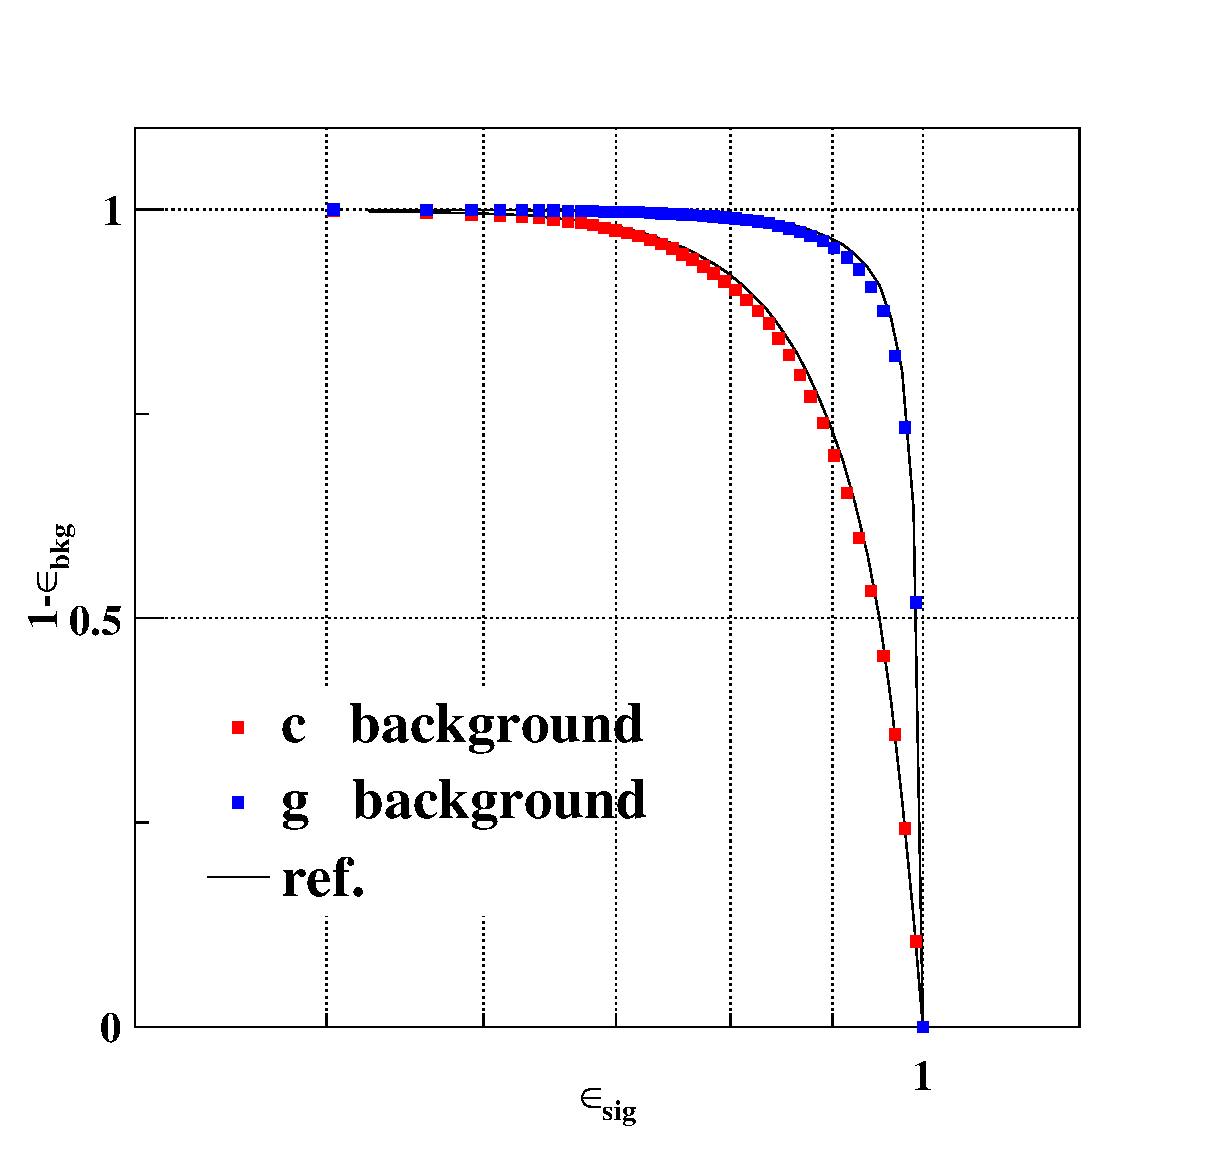
\includegraphics[height=2.4in,width=2.8in,angle=0]{figures/BROC-train.eps}}
	\subfigure[] {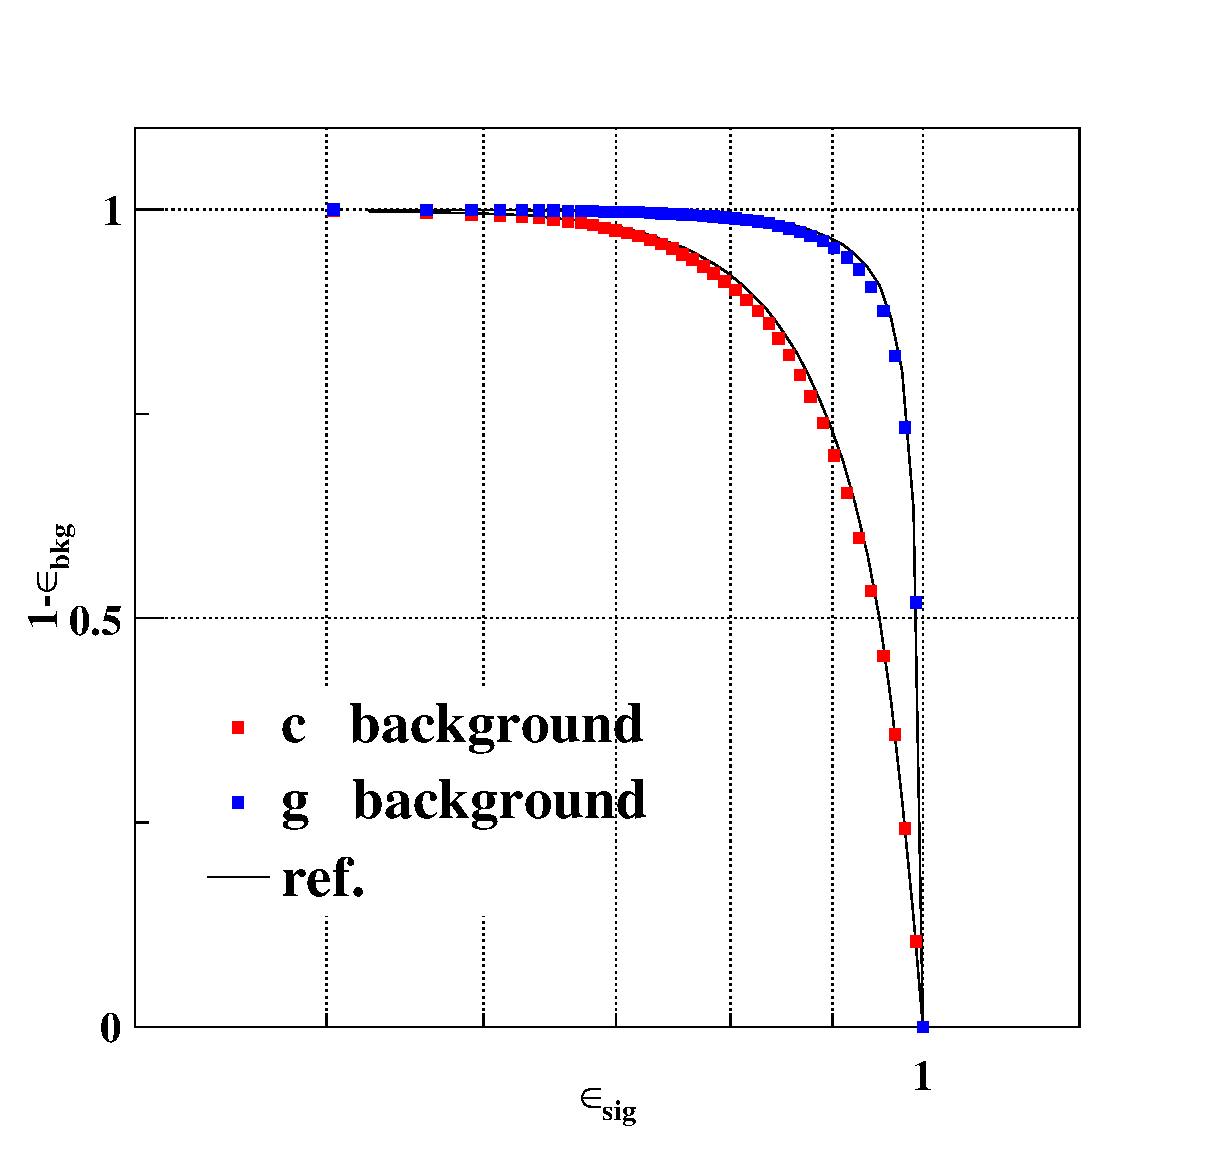
\includegraphics[height=2.4in,width=2.8in,angle=0]{figures/BROC-test.eps}}
	\caption{training (a) and test (b) result of BROC curve for baseline}
	\label{fig:train_test}
\end{figure}


In baseline design, the thickness of silicon sensor is 50um and support is 1mm for the VXD per layer (equivalent to 0.000534 X/$X_0$ and 0.000986 X/$X_0$). Using the command provided by C. FU (/Mokka/init/globalModelParameter VXDSupportScale x; /Mokka/init/globalModelParameter VXDSiliconScale x, while x represents the coefficient related to baseline), we can change the material budget of vertex detector by changing the density of corresponding material. In this work, we change the x from 0.4 to 4. 


The figure \ref{fig:BROC_material} shows the ROC curve of b-quark versus relative material budget. The b-tagging abilities increase with material budget decreasing as we expect. What's more, the reduction of material is inefficient for b-tagging. From the figure \ref{fig:BROC_area}, you can see this result more intuitively. Figure \ref{fig:BROC_area} (a) shows the area below the ROC curve versus relative material budget. For uds background, only 0.5\% relative improvement is seen if we change the relative material budget from 2 to 1. For c background, the improvement is 1\%, very small as well. Figure \ref{fig:BROC_area} (b) shows the purity of b-quark versus relative material budget when b-tagging efficiency is 80\%. There is no obvious critical point for b-tagging and the purity is almost linear with material budget.  For usd backgroud, the purity variation of 0.4\% is found when we change the relative material budget with value of X (X means the baseline material budget). For c backgroud, the purity variation of 2.2\% is found when we change the relative material budget with value of X.
\begin{figure}[!ht]
	\centering
	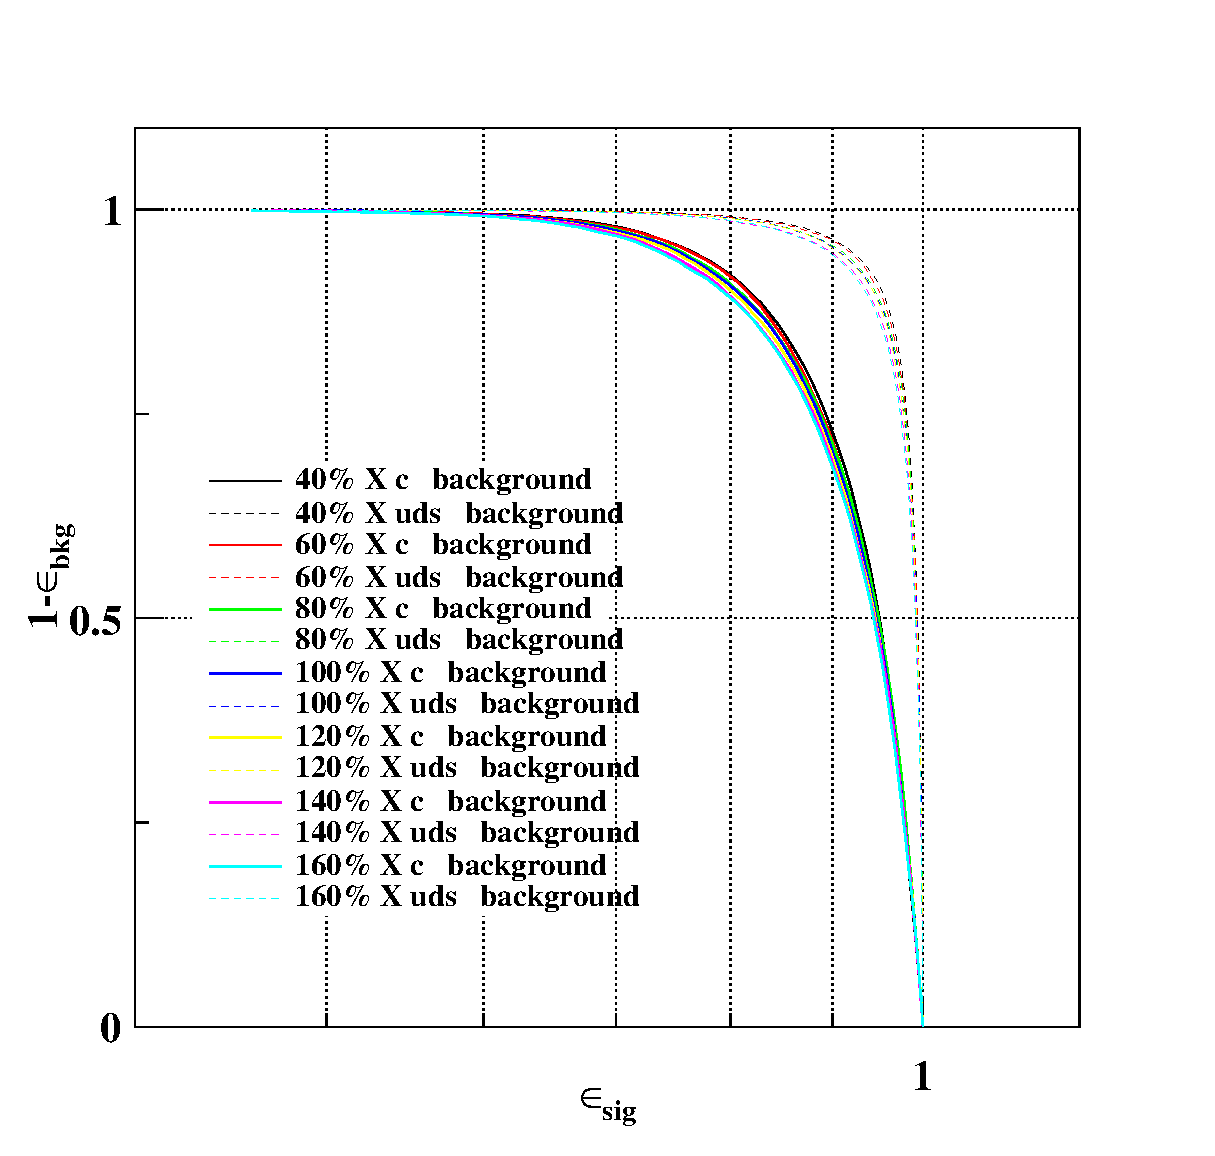
\includegraphics[scale=0.5]{figures/BROC-lcfiweights-test.eps}
	\caption{BROC curve versus relative material budget}
	\label{fig:BROC_material}
\end{figure}

\begin{figure}[!ht]
	\centering
	\subfigure[] {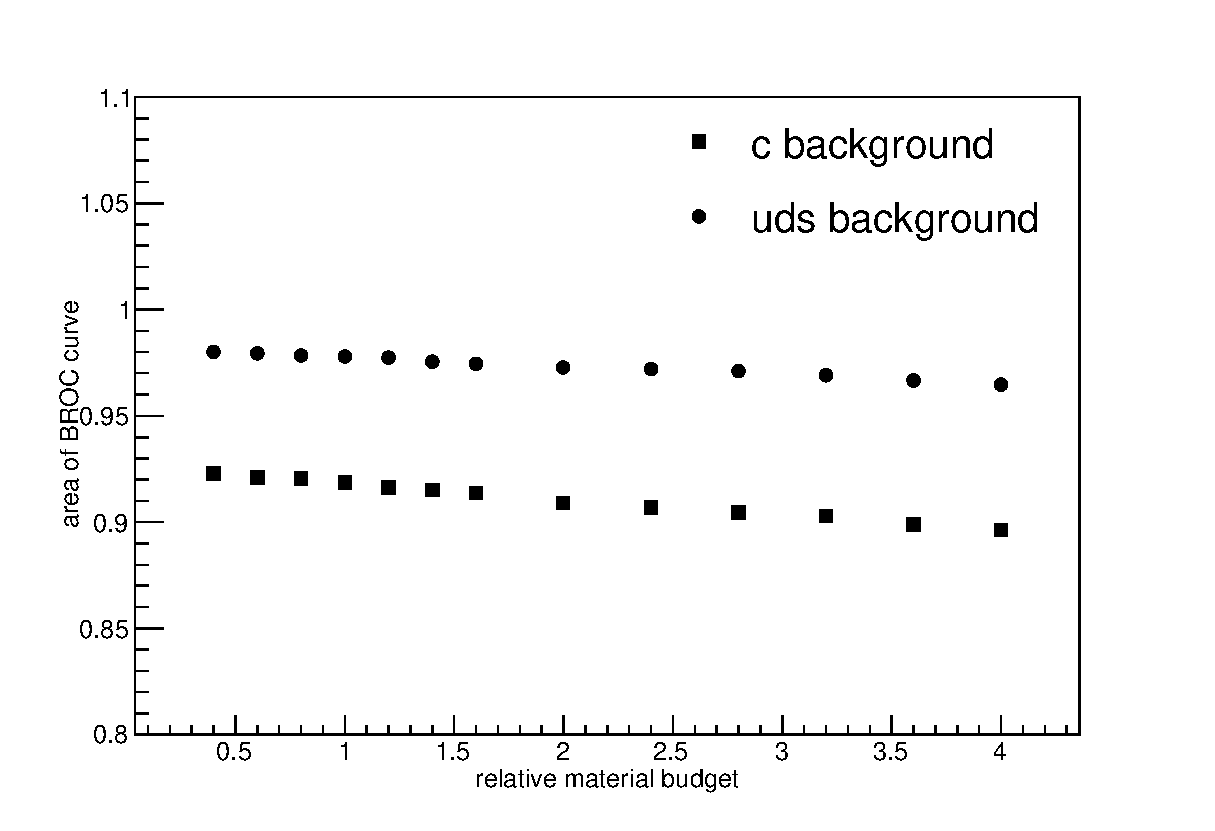
\includegraphics[height=2.4in,width=2.8in,angle=0]{figures/integralB.eps}}
	\subfigure[] {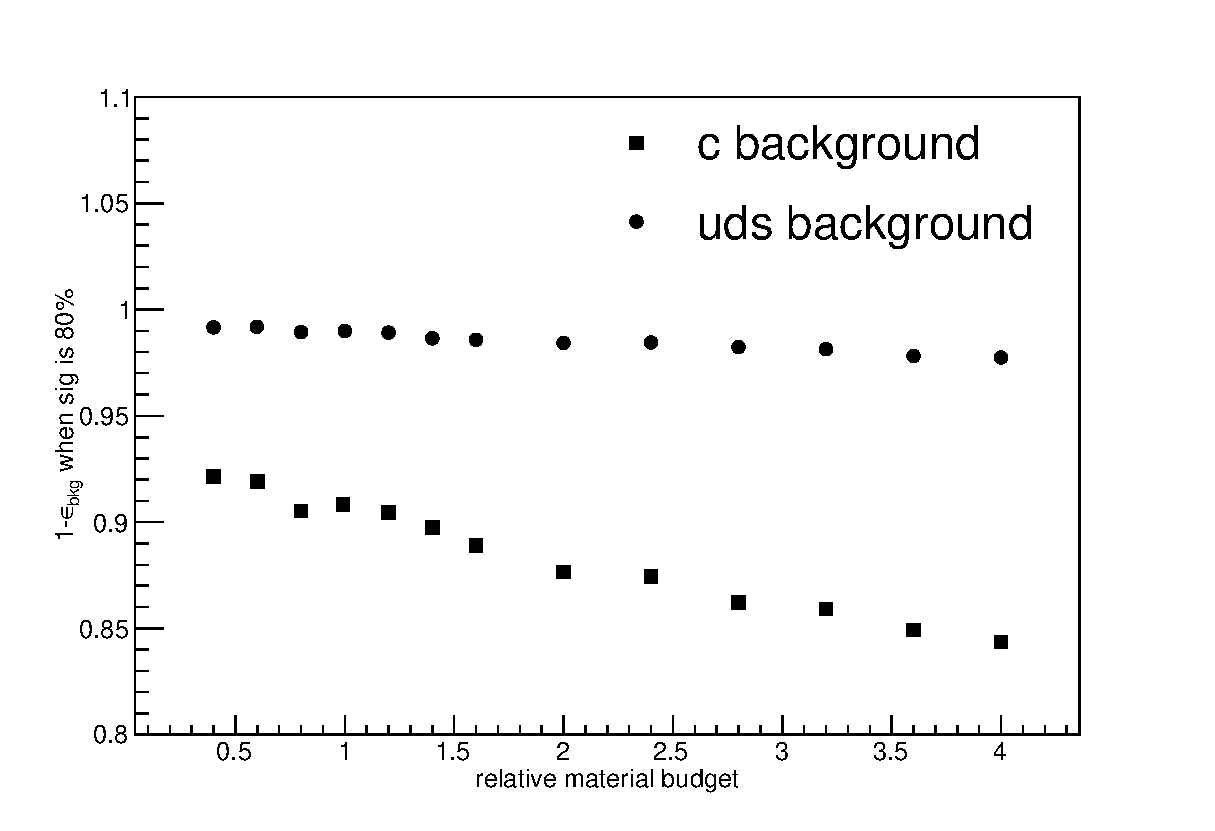
\includegraphics[height=2.4in,width=2.8in,angle=0]{figures/80B.eps}}
	\caption{(a) the area of ROC curve versus relative material budget and (b) rejection efficiency when B-tagging efficiency is 80\% versus relative material budget}
	\label{fig:BROC_area}
\end{figure}


The same thing is done for c-tagging. Figure \ref{fig:CROC_material} shows the CROC curve versus relative material budget. Similar with b-tagging, c-tagging performance improves while material budget decreases. But the different thing is that the reduction of material is much more efficient for c-tagging especially for uds background. Figure \ref{fig:CROC_area} (a) shows the area below the ROC curve versus relative material budget. For uds background, 2\% improvement is seen if we change the relative material budget from 2 to 1. For b background, the improvement is 2\% as well. Figure \ref{fig:CROC_area} (b) shows the purity of c-quark versus relative material budget when c-tagging efficiency is 60\%. There is no obvious critical point for c-tagging and the purity is almost linear with material budget as well.  For usd backgroud, the purity variation of 2.6\% is found when we change the relative material budget with value of X (X means the baseline material budget). For b backgroud, the purity variation of 1.9\% is found when we change the relative material budget with value of X.
\begin{figure}[!ht]
	\centering
	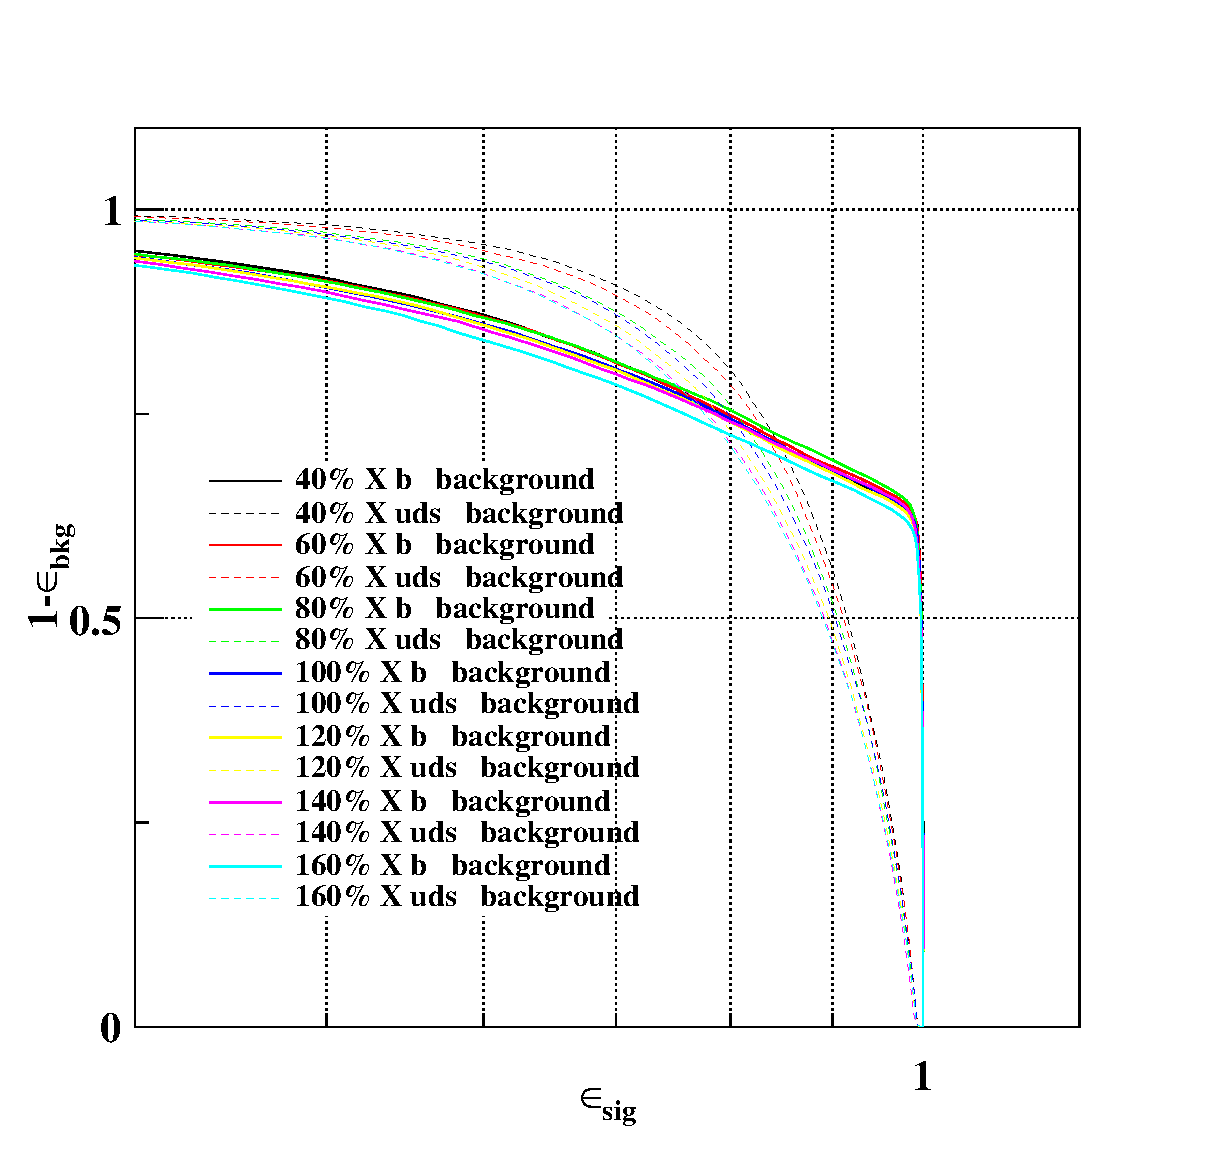
\includegraphics[scale=0.5]{figures/CROC-lcfiweights-test.eps}
	\caption{CROC curve versus relative material budget}
	\label{fig:CROC_material}
\end{figure}

\begin{figure}[!ht]
	\centering
	\subfigure[] {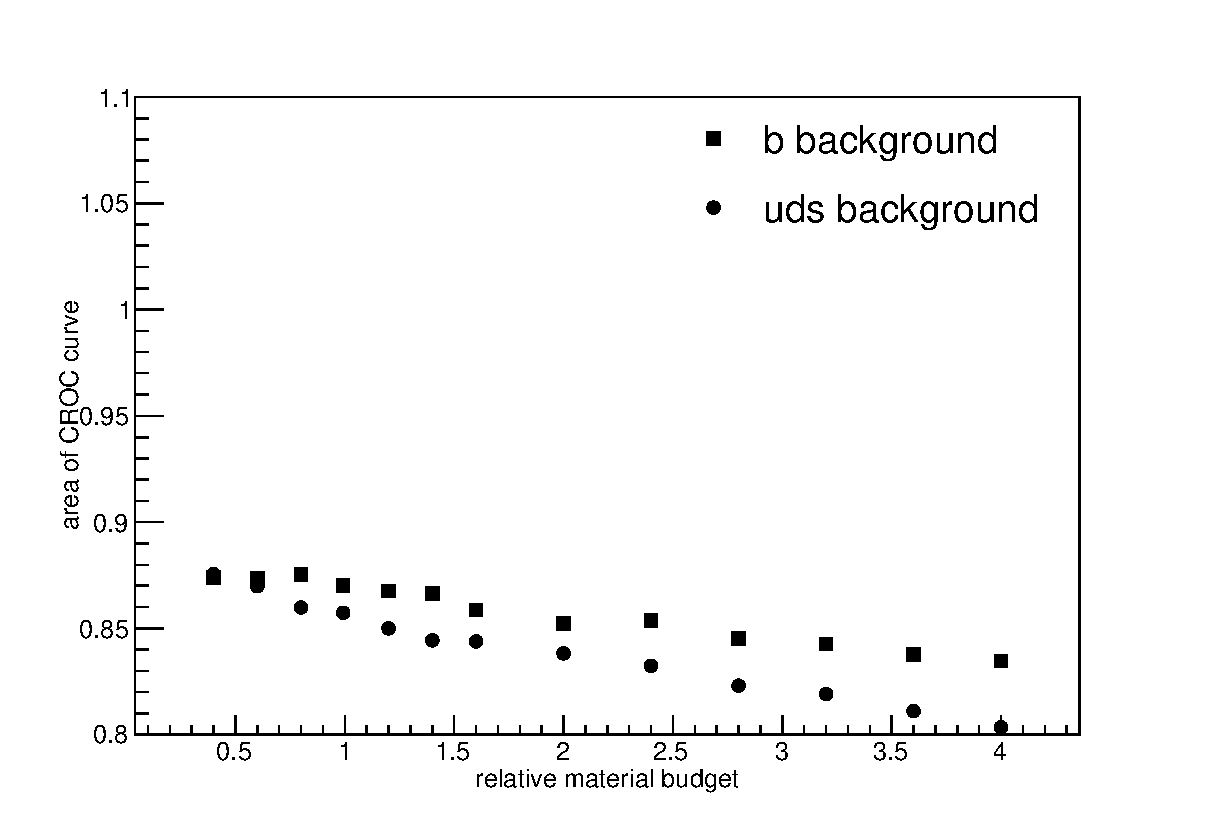
\includegraphics[height=2.4in,width=2.8in,angle=0]{figures/integralC.eps}}
	\subfigure[] {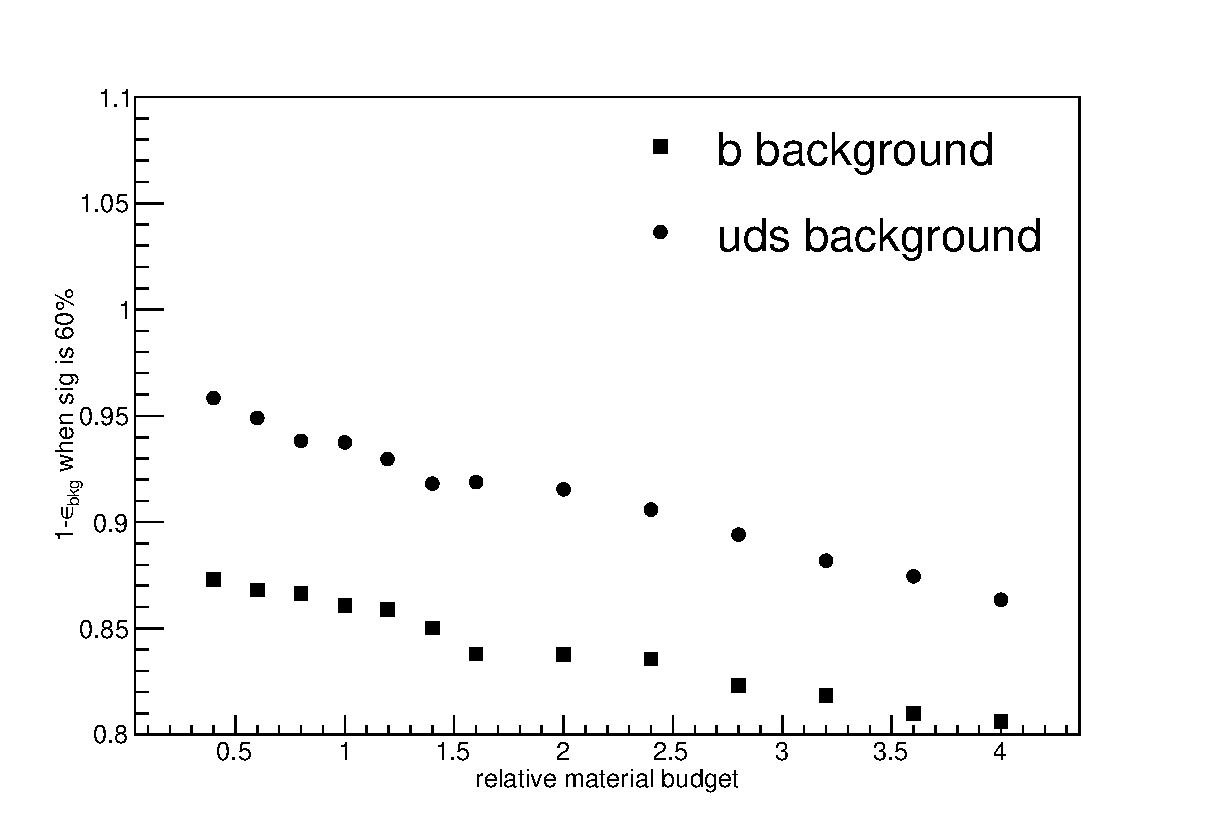
\includegraphics[height=2.4in,width=2.8in,angle=0]{figures/60C.eps}}
	\caption{(a) the area of ROC curve versus relative material budget and (b) rejection efficiency when C-tagging efficiency is 60\% versus relative material budget}
	\label{fig:CROC_area}
\end{figure}


\subsection{Spatial resolution}

In this section, we change the resolution of vertex detector while other parameters remain the same. Here we list the conditions of our simulation below:
\begin{itemize}
	\item default: CEPC\_v1 default setting;
	\item 5\_10: VXD 1-6 and FTD\_pixel 5um, SIT/SET and FTD\_strip 10um
	\item 5\_10\_10: VXD 1 and FTD\_pixel 5um, VXD 2-6 10um, SIT/SET and FTD\_strip 10um
	\item 5\_10\_15: VXD 1 and FTD\_pixel 5um, VXD 2-6 10um, SIT/SET and FTD\_strip 15um
	\item 10\_10: VXD 1-6 and FTD\_pixel 10um, SIT/SET and FTD\_strip 10um
	\item 10\_15: VXD 1-6 and FTD\_pixel 10um, SIT/SET and FTD\_strip 15um
\end{itemize}


The figure \ref{fig:BROC_res} shows b-tagging performance while the figure \ref{fig:CROC_res} shows c-tagging performance. We can see that the smaller the resolution is, the stronger the tagging abilities are. For b-tagging, this phenomenon is not obvious. While for c-tagging, significant improvement is observed.
\begin{figure}[!ht]
	\centering
	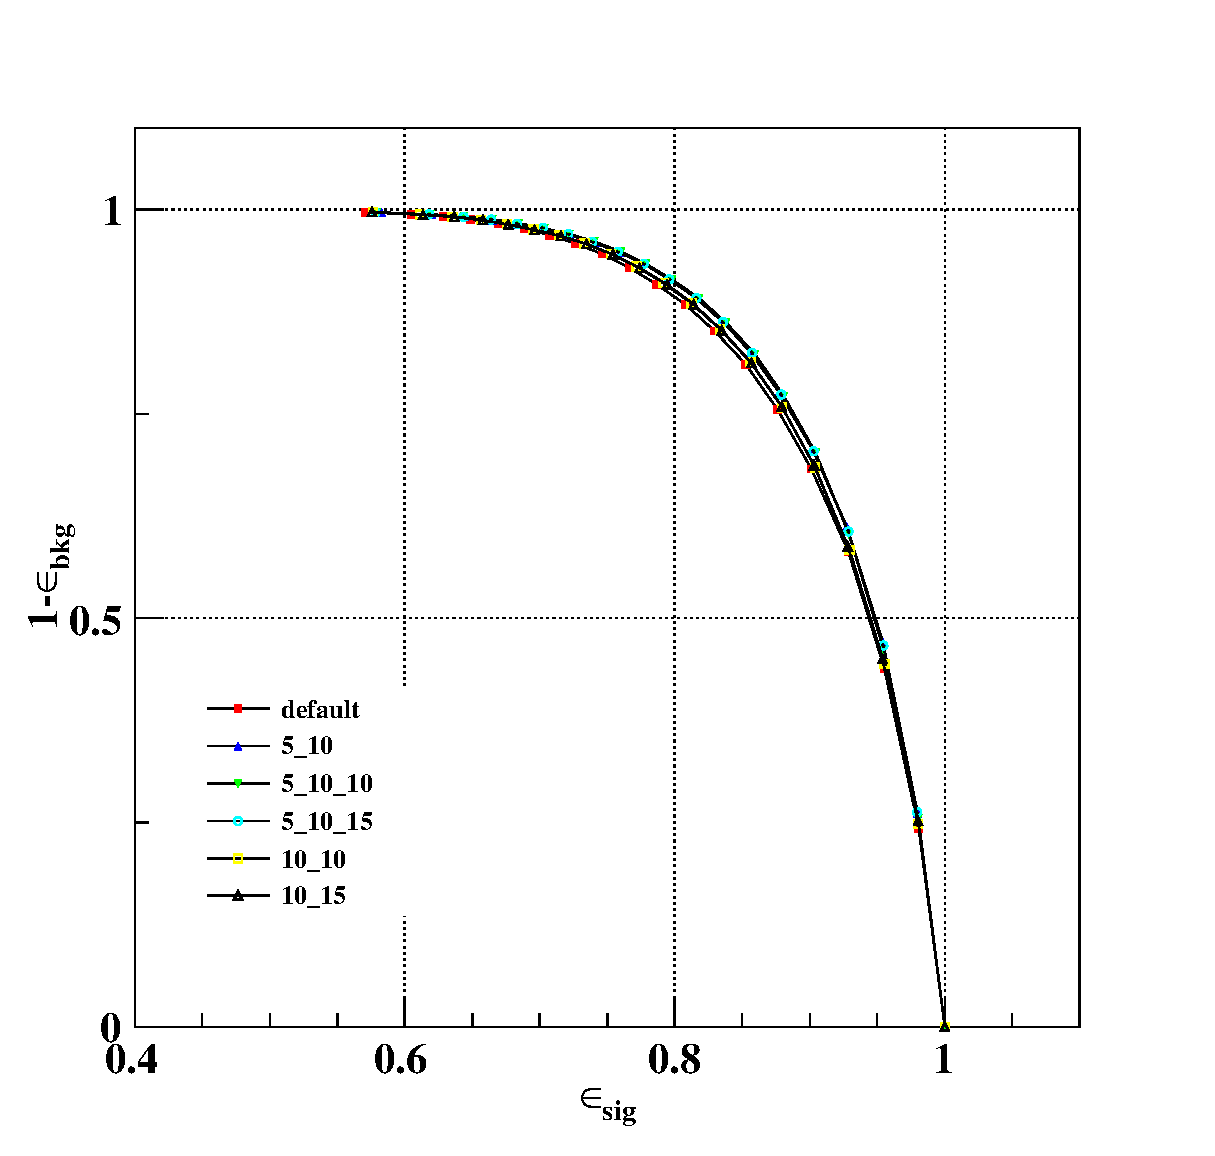
\includegraphics[scale=0.35]{figures/resolution/plot6ROC-cbkg-bjet.eps}
	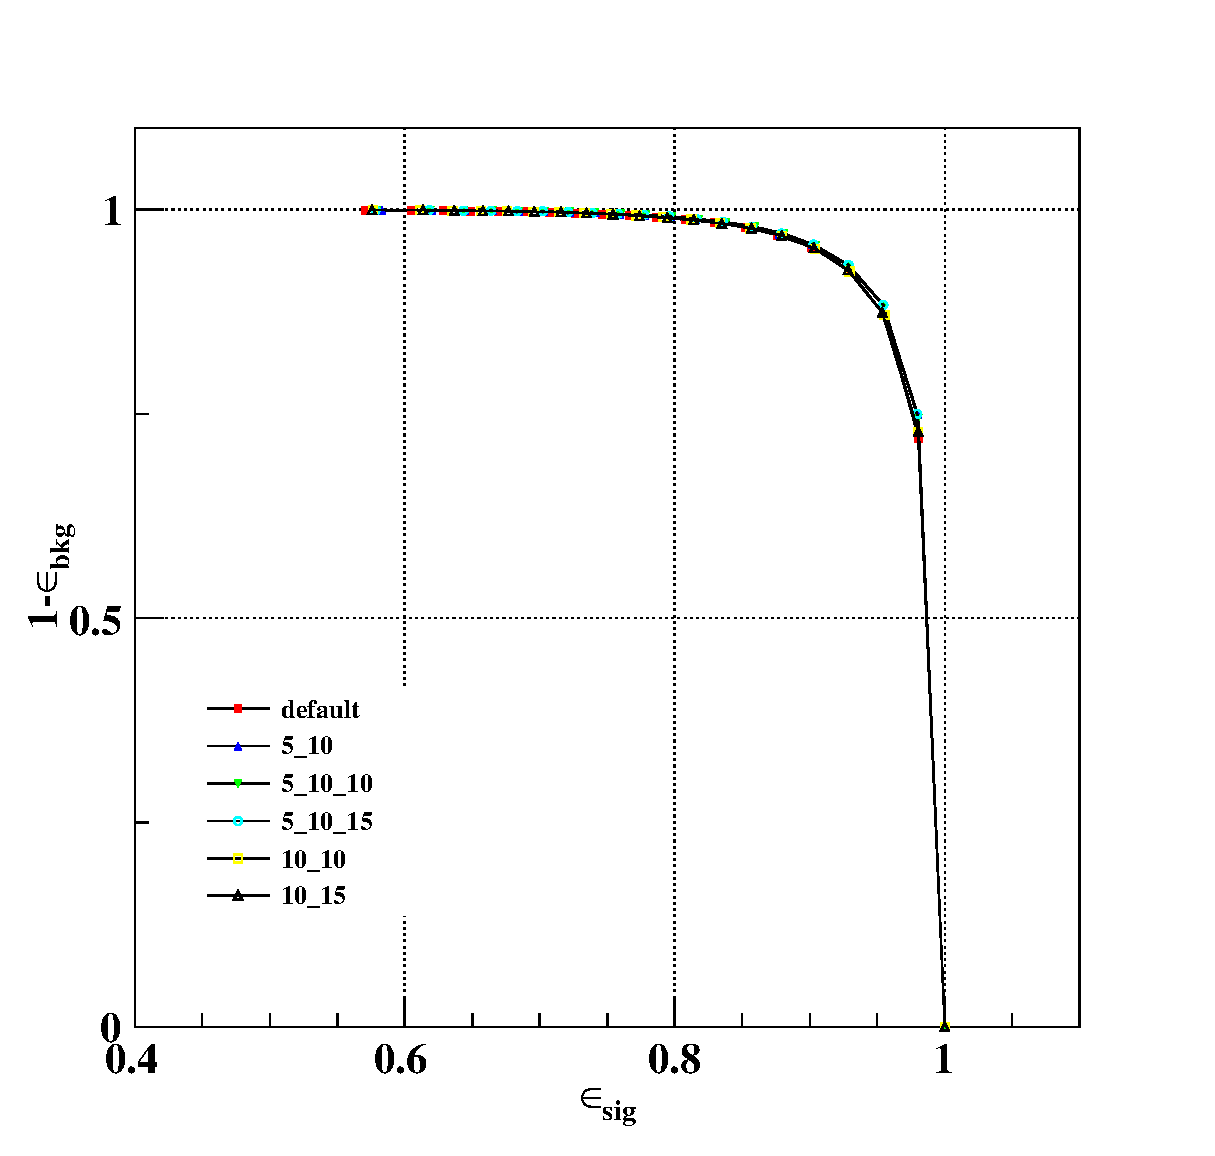
\includegraphics[scale=0.35]{figures/resolution/plot6ROC-obkg-bjet.eps}
	\caption{BROC curve versus different resolution}
	\label{fig:BROC_res}
\end{figure}

\begin{figure}[!ht]
	\centering
	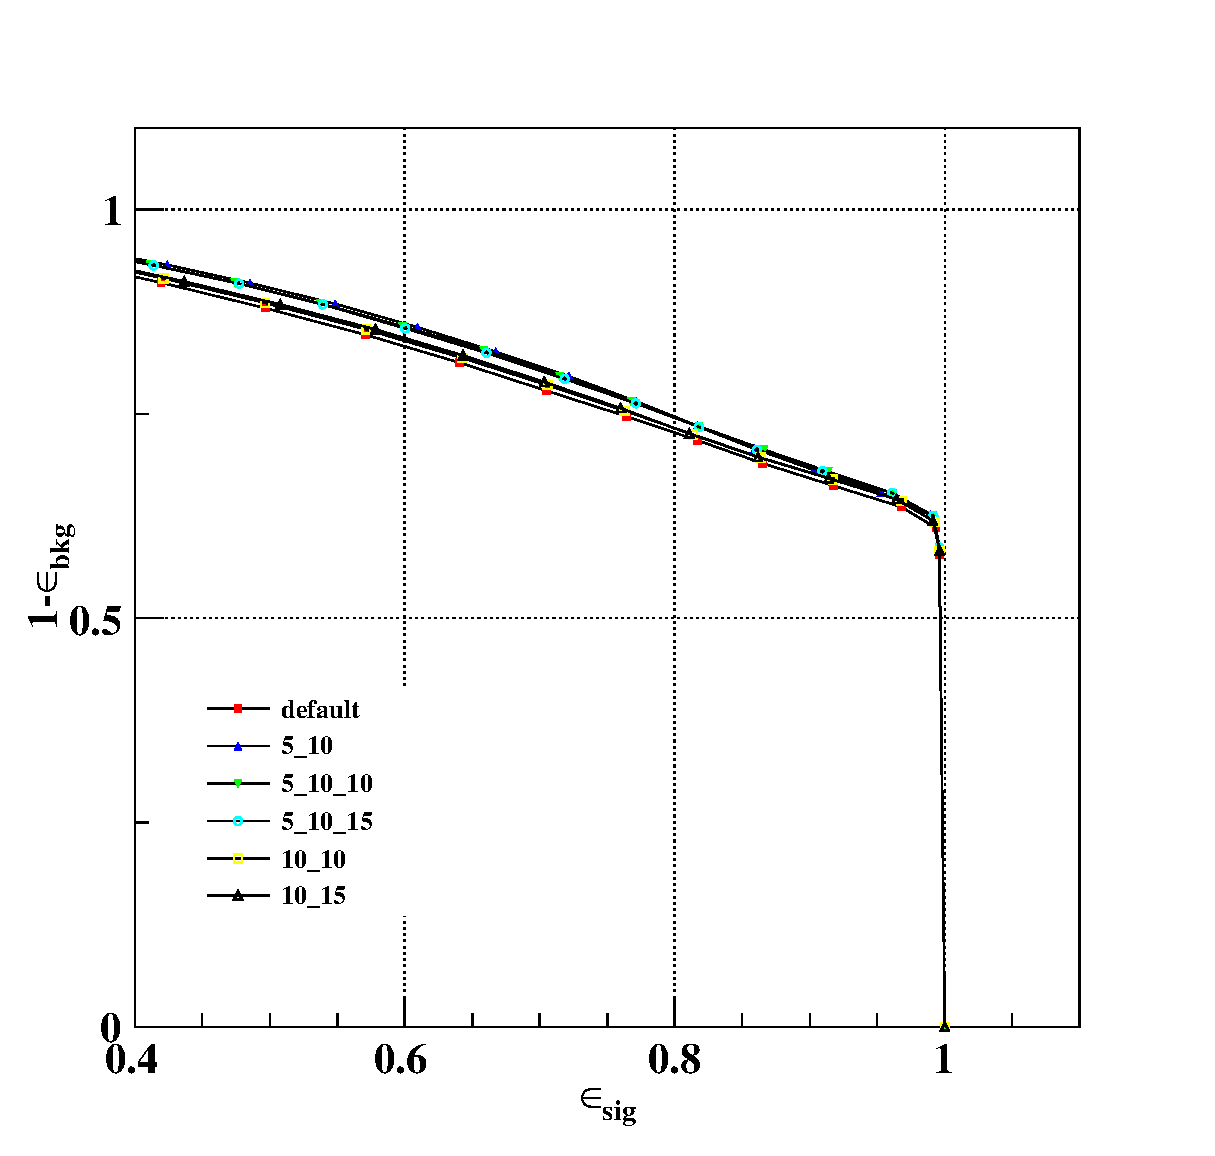
\includegraphics[scale=0.35]{figures/resolution/plot6ROC-bbkg-cjet.eps}
	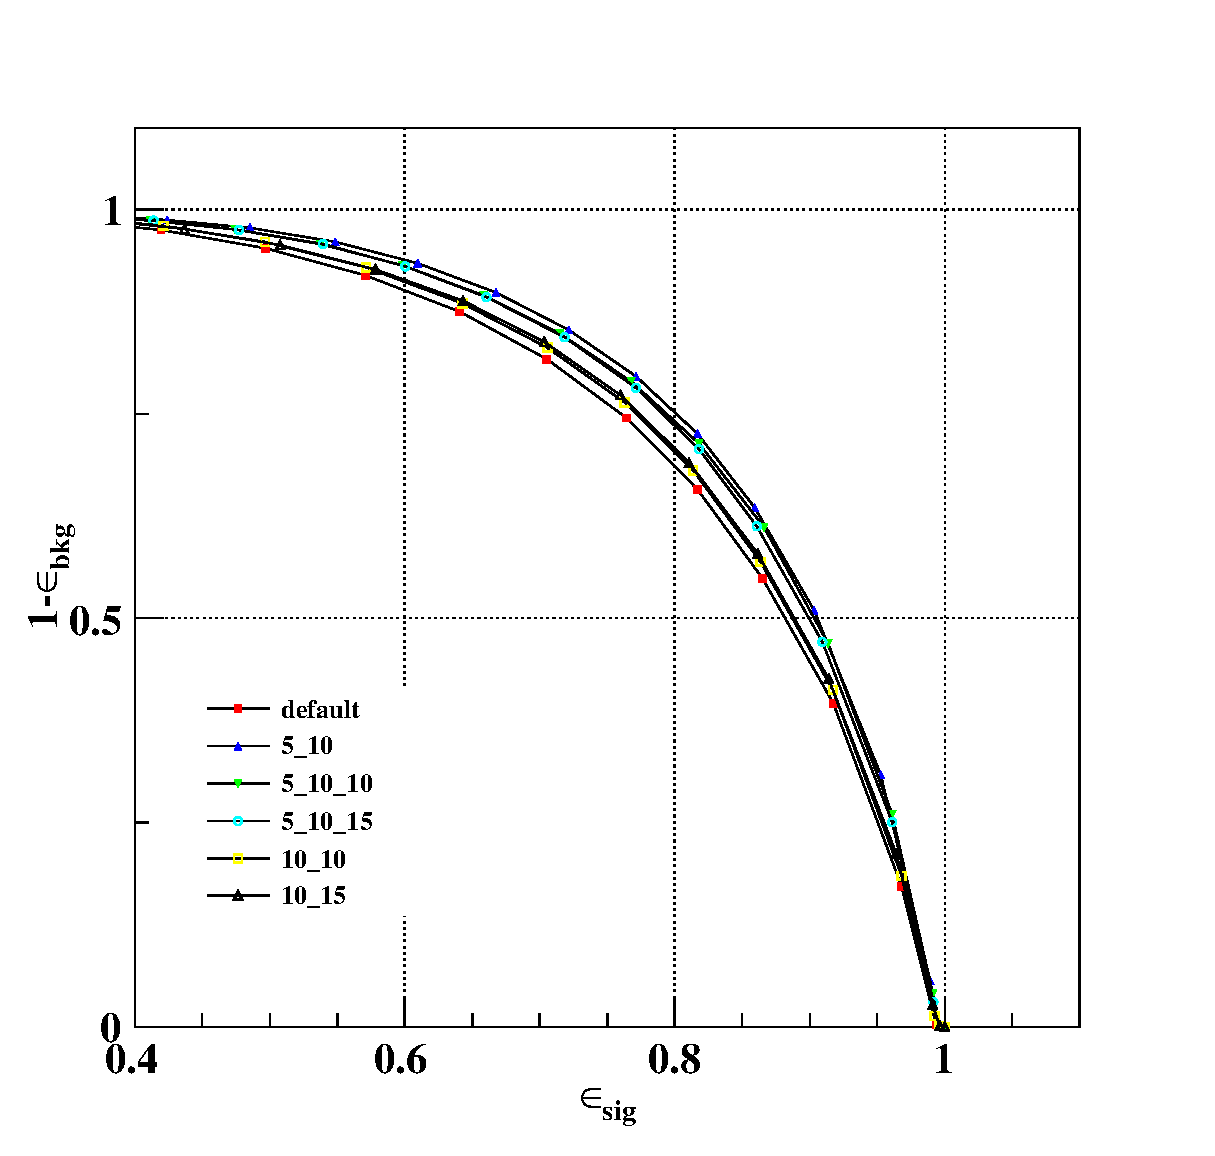
\includegraphics[scale=0.35]{figures/resolution/plot6ROC-obkg-cjet.eps}
	\caption{CROC curve versus different resolution}
	\label{fig:CROC_res}
\end{figure}

\subsection{Inner resolution}

In this section, we change the radius of innermost layer with the value of 8mm, 10mm, 12mm, 14mm, 16mm and 20mm. 
The figure \ref{fig:ROC_radius_b} and \ref{fig:ROC_radius_c} show the ROC curve of b-tagging and c-tagging. It reflects that pushing vertex to IP improves c-tagging significantly.
\begin{figure}[!ht]
	\centering
	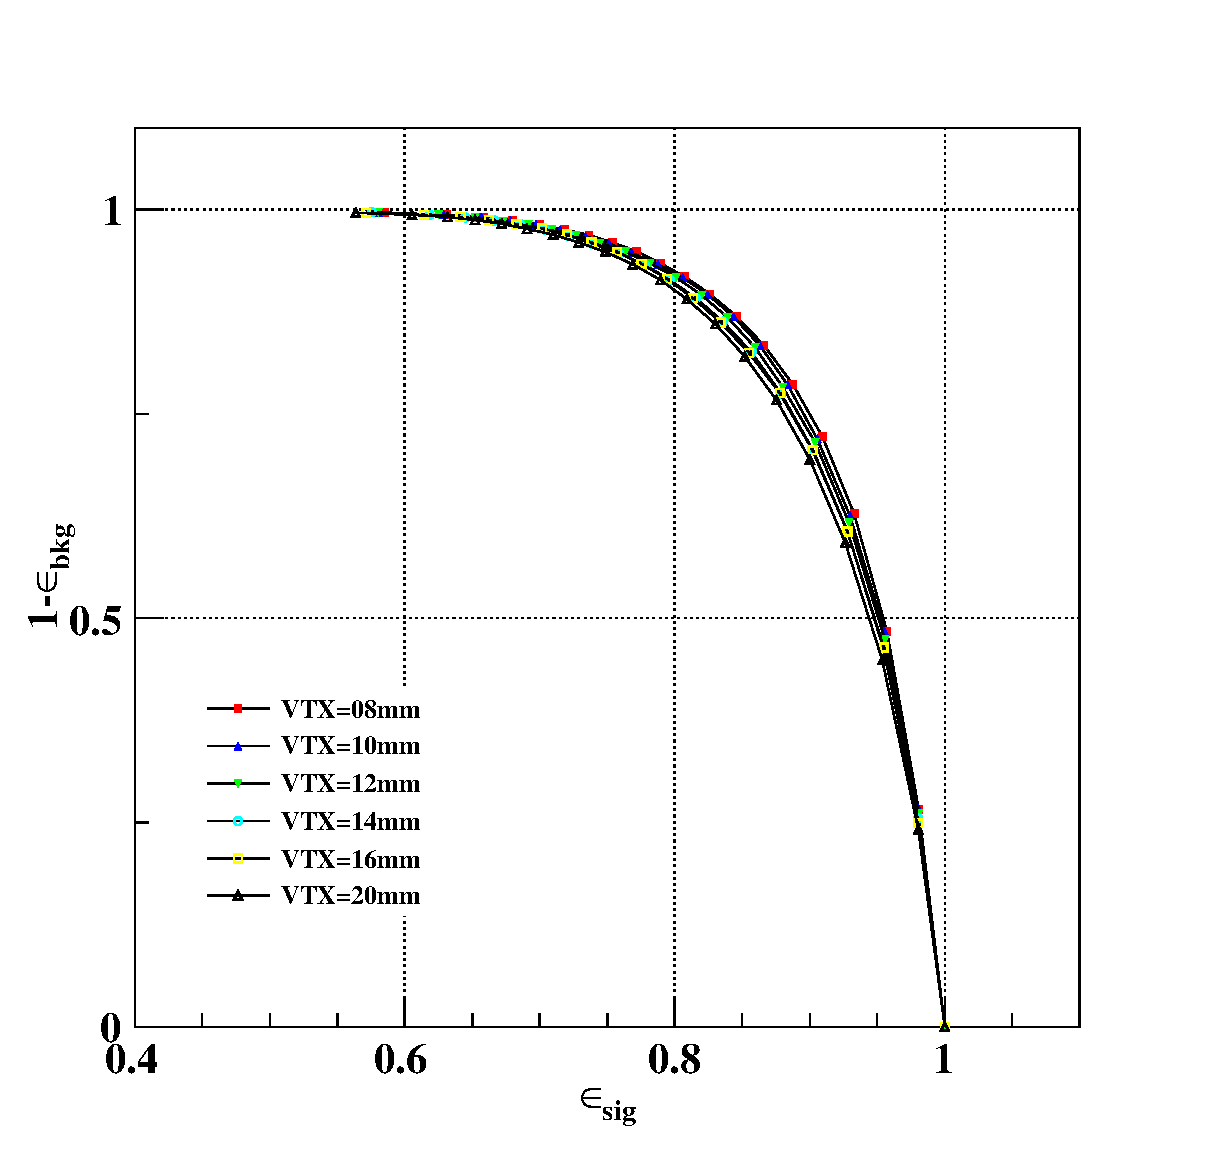
\includegraphics[scale=0.35]{figures/radius/plot6ROC-cbkg-bjet.eps}
	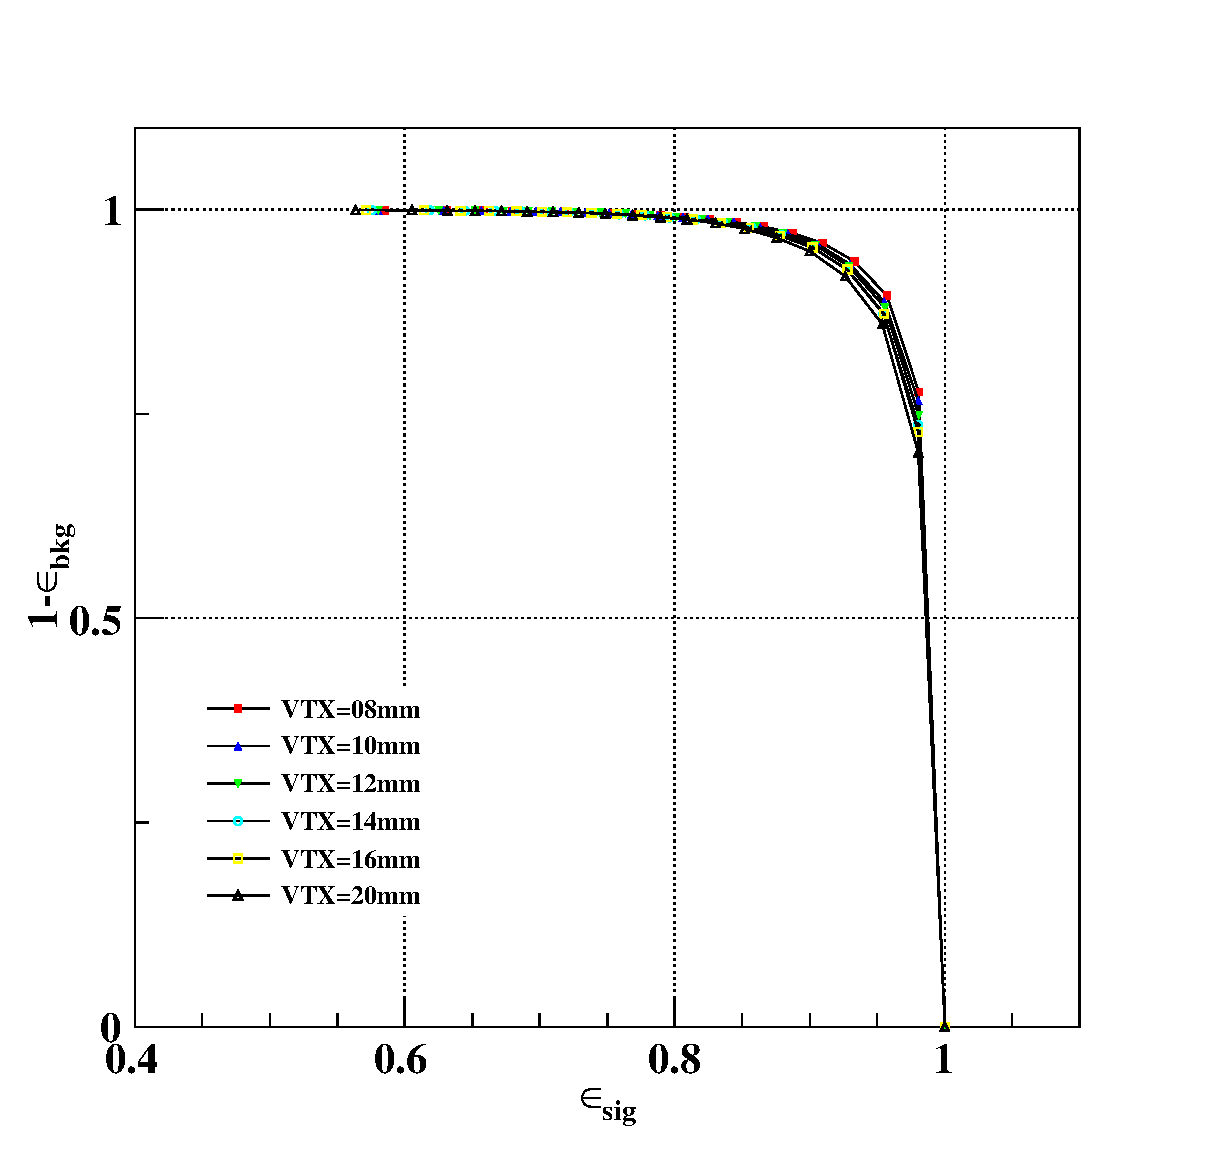
\includegraphics[scale=0.35]{figures/radius/plot6ROC-obkg-bjet.eps}
	\caption{BROC curve versus different inner radius }
	\label{fig:ROC_radius_b}
\end{figure}

\begin{figure}[!ht]
	\centering
	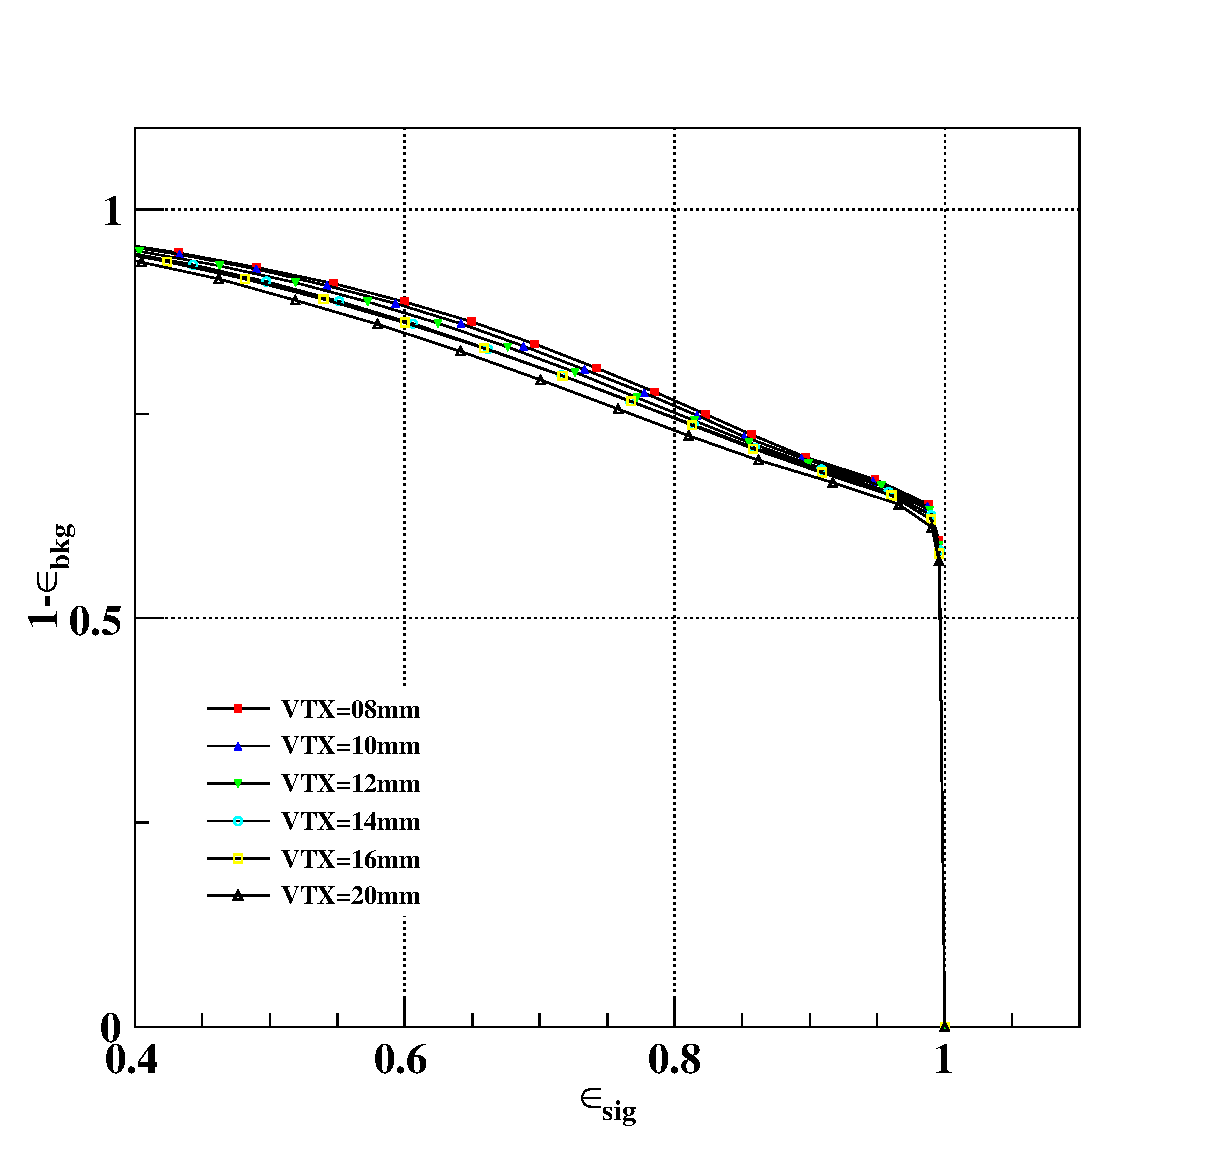
\includegraphics[scale=0.35]{figures/radius/plot6ROC-bbkg-cjet.eps}
	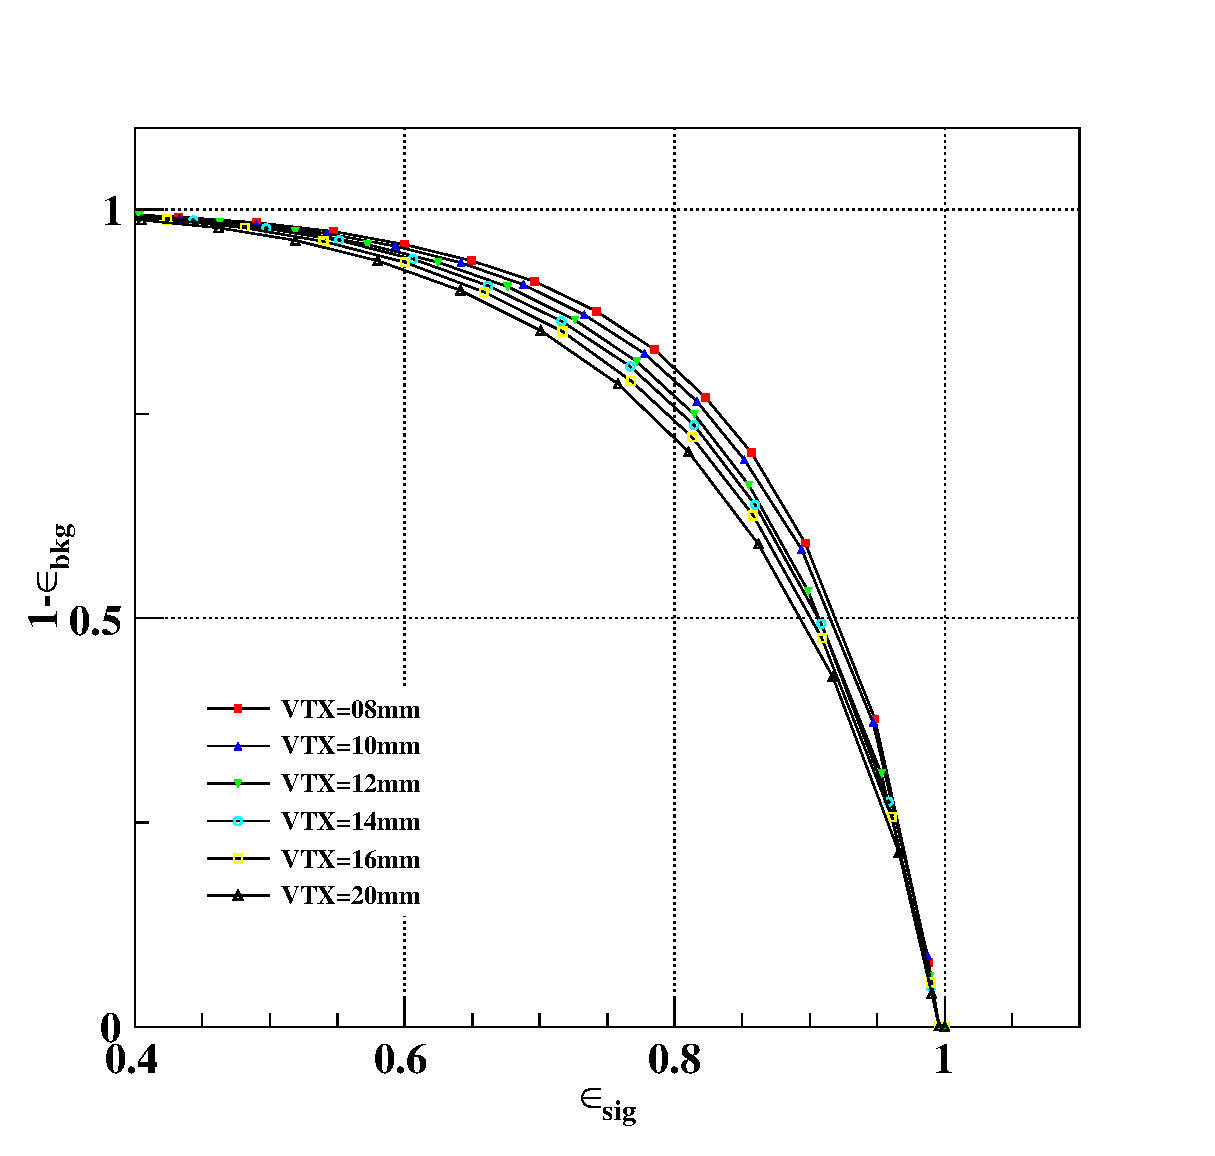
\includegraphics[scale=0.35]{figures/radius/plot6ROC-obkg-cjet.eps}
	\caption{CROC curve versus different inner radius}
	\label{fig:ROC_radius_c}
\end{figure}
\section{Conclusion}

We have done the optimization of material budget, spatial resolution and inner radius for CEPC vertex detector. 
The results are reasonable and consistent with each other. 
We can conclude that the optimization of vertex improves c-tagging significantly, while has small influence on b-tagging. 
In detail, decreasing the material budget of vertex detector contributes a better distinction of b-quark and c-quark,
which is about 1.4\% purity improvement with 0.001$X/X_0$ material reduction. 
For uds, the optimization of material budget make more sense for c-tagging than b-tagging, 
which is about 1.7\% improvement with 0.001$X/X_0$ material reduction for c-tagging and 0.27\% improvement with 0.001$X/X_0$ material reduction for b-tagging.

\end{document}
